Consider a typical loss development context, where
a large set of homogeneous insurance risks (e.g. private
car insurance policies) are aggregated
into a loss triangle with
cumulative loss amounts denoted
$\mathcal{Y}$, defined by:

\begin{equation}
	\mathcal{Y} = \{y_{ij} : i = 1, ..., N; j = 1, ..., N - i + 1\}
\end{equation}
%
where $i = 1, ..., N$ denotes experience periods 
indexing all claims occurring during period $i$, and $j = 1, ..., M$
denotes development periods. 
Most frequently, $N = M$.
For a particular point in time,
development information for period $i$ is only known up to period 
$j = N - i + 1$,
and therefore $\mathcal{Y}$ represents the left upper diagonal of
the loss triangle. The complementary, lower diagonal 
triangle, denoted $\tilde{\mathcal{Y}}$,
with $\frac{N (M - 1)}{2}$ entries 
for a square matrix,
is unknown and the goal of prediction.

The generative process considered here (Figure \ref{fig:schematic})
is that cumulative losses
in $\mathcal{Y}$ develop according to $i$) a period that is
characterised by largely, but not strictly, monotonically 
increasing losses 
(the body), followed by $ii$) a period of smooth
growth to ultimate (the tail). Traditional methods
treat estimation of body and tail as a two-step process.
By contrast, the hidden Markov development model introduces a
latent, discrete state $\bm{z} = (z_{11}, z_{12}, ..., z_{ij}, ..., z_{NM})
\in \{1, ...,  K\}$, with $K = 2$, that takes value
$z_{ij} = 1$ if the body process generated the losses in the $i$th
accident period and $j$th development period, and
$z_{ij} = 2$ if the tail process generated the losses.
The latent state at one time point, $z_{ij}$, is dependent
on the state at the previous time point, $z_{ij-1}$,
and subsequent states are connected via a state transition
matrix, $\Theta_{ij}$.
Depending on the latent state and any other parameters
$\bm{\phi}$, the likelihood, $p(y_{ij} \mid z_{ij}, \bm{\phi})$,
is given by suitable \textit{emission} distributions.
Emission distributions are the observation data distributions,
which in loss development modelling are typically
positive-bound, continuous probability density
functions, such as lognormal or Gamma.
In this paper, all models use lognormal distributions
as the likelihood distribution.

\begin{figure}[t!]
    \centering
    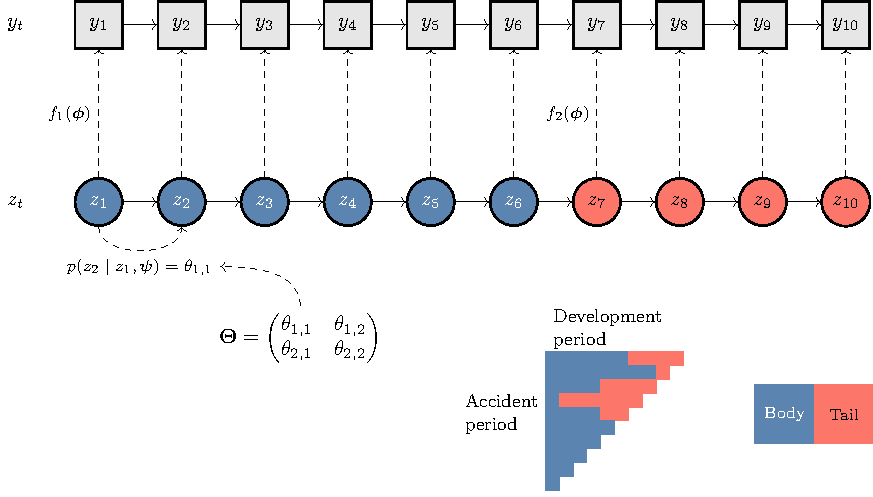
\includegraphics[scale=0.9]{\figures/figure1.pdf}
    \caption{
        A schematic of the hidden Markov model process.
        A loss triangle of observed data is shown
        with 10 accident periods. Observed losses
        at each development period and accident period
        is generated from one of
        two processes: the body (blue)
        and or tail (orange). The dynamics of the
        body and tail states vary over accident periods.
        For the first accident period, $y_{1j}$,
        the hidden Markov process is illustrated
        across development periods $j = 1, ..., 10$.
        Observed losses are shown as grey
        squares and are assumed generated from the latent
        discrete random variable $z_{1j}$ (circles) via
        emission distributions.
        Latent states transition according
        to the probabilities
        in matrix $\Theta_{1j}$, depending on parameters
        $\bm{\psi}$, and $\mu_{1_{1j}}$ and $\mu_{2_{1j}}$
        represent the body and tail state emission distributions.
   }
	\label{fig:schematic}
\end{figure}

The hidden Markov development model can be
written generally as:

\begin{align}
	\begin{split}
	\label{eq:hmm}
	y_{ij} &\sim \begin{cases}
        \mathrm{Lognormal}(\mu_{1_{ij}}, \sigma_{ij}) \quad z_{ij} = 1\\
        \mathrm{Lognormal}(\mu_{2_{ij}}, \sigma_{ij}) \quad z_{ij} = 2\\
	\end{cases}\\
    z_{ij} &\sim \mathrm{Categorical}(\Theta^{z_{ij-1}}_{ij})\\
    \Theta_{ij} &= \begin{pmatrix}
        \pi & 1 - \pi\\
        \nu & 1 - \nu
    \end{pmatrix}\\
    \log \frac{\pi}{1 - \pi} &\sim \mathrm{Normal}(0, 1)\\
    \log \frac{\nu}{1 - \nu} &\sim \mathrm{Normal}(0, 1)\\
	\end{split}
\end{align}
%
The cumulative losses at accident period $i$ and development period $j$
are assumed positive-bound, lognormally-distributed random variates,
with log-scale location $\mu_{1_{ij}}$ if the process is in the body
or $\mu_{2_{ij}}$ if the process is in the tail, and with scale $\sigma_{ij}$.
The latent state $z_{ij}$ determines the body or tail state at each
time point, and follows a categorical distribution with unit simplex probabilities
determined by row $z_{ij - 1}$ of the state transition matrix, shown
by the superscript in $\Theta_{ij}^{z_{ij - 1}}$. 
As discussed below, the state transition matrix
may be time-homogeneous or -inhomogeneous, depending on the context.
In the state-transition matrix, 
$\pi$ denotes $p(z_{ij} = 1 \mid z_{ij-1} = 1)$, the 
probability of staying in the body
process at period $j$, and $\nu = p(z_{ij} = 2 \mid z_{ij-1} = 2)$,
the probability of staying in the tail at period $j$.
Their complements, $1 - \pi$ and $1 - \nu$, represent the
probabilities of transitioning from body to tail, and tail
to body, respectively.

The emission distributions, $\mu_{1_{ij}}, \mu_{2_{ij}})$,
used here are two canonical body and tail development models:
the chain ladder model for body loss development factors
\citep{mack1993,englandverrall2002},
and an exponential decay curve following the generalised Bondy model
for the tail process \citep{tailfactors2013}.
The full model specification is completed by choosing these
functional forms, along with the functional form for the variance
and the remaining prior distributions.

\begin{align}
\begin{split}
    \mu_{1_{ij}} &= \log(\alpha_{j - 1} y_{ij-1}) \quad \forall j > 1\\
    \mu_{2_{ij}} &= \log(\omega^{\beta^{j}} y_{ij - 1}) \quad \forall j > 1\\
	\sigma_{ij}^2 &= \exp(\gamma_{1} + \gamma_{2} j + \ln(y_{ij-1}))\\
	\log \bm{\alpha}_{1:M - 1} &\sim \mathrm{Normal}(0, 1 / 1:M - 1)\\
    \log \omega &\sim \mathrm{Normal}(0, 1)\\
    \log \frac{\beta}{1 - \beta} &\sim \mathrm{Normal}(0, 1)\\
    \bm{\gamma}_{1:2} &\sim \mathrm{Normal}(0, 1)\\
\end{split}
\end{align}
%
Due to the multiplicative autoregressive nature of typical
loss development models, the first data point is not modelled,
and the hidden Markov process is assumed to start in the
body state.
The $M - 1$ body link ratios are given by the vector $\bm{\alpha}$,
and the tail link ratios are given by $\omega^{\beta^{j}}$, for any $j$,
allowing extrapolation out to arbitrary development periods.
The parameter $\omega$ is constained to be strictly greater than $1.0$,
such that growth is monotonically increasing,
and $\beta$ is constrained to lie in the interval $(0, 1)$, to avoid
tail factors growing without bound to $\infty$.
The expression for the variance encodes the assumption of
less volatility at higher development periods, and is proportional
to the losses at the previous time point.

The prior distribution on $\bm{\alpha}$ is regularised towards
a link ratio of 1 in inverse proportion to the development period.
This assumption is imposed to ensure link ratios, 
when $z_{ij} = 2$ (i.e. the latent state 
is in the tail process), do not become unrealistically
large due to the resulting non-identifiability. 
Even when the tail process
is most likely,
some samples could be generated from the body process because
$z_{ij}$ is a random variable, and large values of $\alpha_{ij-1}$
might have unwanted influence on the predictions.
This is akin to the use of pseudo-priors in Bayesian mixture
models \citep{carlinchib1995}, which ensure parameters in the mixture
not being sampled do not become implausible.

\subsection{Model variants}
Three variations of the hidden Markov model are used (Table \ref{table:variants}). 
The base model (referred to as HMM) has homogeneous transition matrix $\Theta$,
and sets $\nu$ to zero. This implies that once the tail
process is active, the model cannot switch back to the
body process. This is the primary assumption underlying
tail modelling generally: at some development point, the 
losses smoothly develop to ultimate. Secondly, the HMM-$\nu$
model estimates $\nu$, allowing for tail processes to switch
back to body processes. Some triangles may illustrate
unexpected late-development volatility, at which point
the more flexible body process is a better explanation
of the data. Finally, the HMM-lag variant allows $\pi$
to vary across development periods, $\bm{\pi} = (\pi_{1}, 
..., \pi_{j - 1}, ..., \pi_{M - 1})$, on which 
an ordered assumption is imposed such that the probability
of transitioning to the tail increases with development period,
meaning $\pi_{j - 1} < \pi_{j - 2}$.
Many extensions of these variants are possible, including
the addition of covariates on the estimation of
$\Theta$ or other parametric or non-parametric
forms. This paper restricts focus on these three
variants as they present the simplest use cases
to compare to the two-step process. Although
the HMM-lag and HMM-$\nu$ variant could be combined,
early tests of the hidden Markov development model
by the author indicated that this model risked unidentifiability
without further data or covariates.

\begin{table}
    \centering
    \begin{tabular}{p{3cm}|p{3cm}}
        Name & $\Theta_{ij}$ \\
        \hline\\
        HMM & $\begin{pmatrix} \pi & 1 - \pi \\ 0 & 1 \end{pmatrix}$ \\
        HMM-$\nu$ & $\begin{pmatrix} \pi & 1 - \pi \\ \nu & 1 - \nu \end{pmatrix}$\\
        HMM-lag & $\begin{pmatrix} \pi_{ij-1} & 1 - \pi_{ij-1} \\ 0 & 1 \end{pmatrix}$\\
    \end{tabular}
    \caption{
        The three hidden Markov model transition matrix variants
        used in the examples.
    }
    \label{table:variants}
\end{table}

\subsection{Estimation}
The models were fit Stan \citep{stan2017} using Bayesian inference
via Hamiltonian Monte Carlo, via the \texttt{cmdstanpy} \citep{cmdstanpy2024}
Python package and \texttt{cmdstan} \citep{cmdstan2024}. Stan requires specifying a statement
proportional to the joint log density of the data and parameters.
For the above model, the log joint density for a single data point,
grouping all transition matrix parameters as $\bm{\psi} = \{\pi, \nu\}$
and emission distribution parameters as $\bm{\phi} = \{\alpha,
\omega, \beta, \gamma\}$, can be factored as:

\begin{equation}
p(y_{ij}, z_{ij}, z_{ij-1}, \bm{\phi}, \bm{\psi}) = 
    p(y_{ij} \mid  z_{ij}, \bm{\phi})
    p(z_{ij} \mid z_{ij-1}, \bm{\psi})
    p(z_{ij-1} \mid \bm{\psi})
    p(\bm{\psi})
    p(\bm{\phi})
\end{equation}
%
Stan's use of Hamiltonian Monte Carlo means it cannot
directly estimate the discrete parameters 
$z_{ij}$ or $z_{ij-1}$, meaning they
must be marginalised out of the model statement.
Indeed, marginalisation is often more computationally
efficient and stable than estimating discrete parameters
directly.
However, naive marginalisation schemes are inefficient
because the number of possible states increases
exponentially with the number of time points,
providing all states can be transitioned between
at each time point. Therefore, the hidden Markov
models were estimated using the forward algorithm
\cite{rabiner1989},
which iteratively stores the joint probability
of the data and discrete parameter possibilities
across development periods for easy marginalisation. 
The log joint density for a single accident year under
this scheme is:

\begin{equation}
    p(y_{1:M}, \bm{\phi}, \bm{\psi}) = p(y_{iM}, y_{i,1:M-1} \mid \bm{\phi}, \bm{\psi})
    p(\bm{\phi}) p(\bm{\psi})
\end{equation}
%
where $y_{iM}$ are the losses at the
last development period for accident period $i$
and $y_{i,1:M-1}$ are all losses for accident period $i$ up to 
development period $M - 1$. The joint
density of these two terms marginalises
across latent states using the expression:

\begin{align}
    \begin{split}
        p(y_{iM}, y_{i,1:M-1} \mid \bm{\phi}, \bm{\psi}) =
        &\sum_{k=1}^{K} p(y_{ij} \mid z_{ij} = k, \bm{\phi})\\
        &\sum_{h=1}^{K} p(z_{ij} = k \mid z_{ij-1} = h, \bm{\psi})
            p(z_{ij - 1} = h, y_{i, 1:j})
    \end{split}
\end{align}
%
After model fitting, the hidden states on the
training data can be recovered using the
Viterbi algorithm \citep{rabiner1989},
which provides the most likely joint
sequence of latent states that generated
the data. For future data, new samples of
$z_{ij}$ can be taken from a categorical
distribution with estimated parameters of
the transition matrix $\Theta_{ij}$ for
that data point.
